\documentclass[titlepage, 12pt]{article}

\usepackage[margin=1.25in]{geometry}
\usepackage{fancyhdr}
\pagestyle{fancy}

\usepackage{graphicx}

\usepackage{float}
\restylefloat{table}

\usepackage{bookmark}
\bookmarksetup{
  open,
  depth=2
}

\newenvironment{packed_itemize}{
  \vspace{-\topsep}
  \begin{itemize}
    \setlength{\itemsep}{1pt}
    \setlength{\parskip}{0pt}
    \setlength{\parsep}{0pt}
  }{\end{itemize}}

\newcommand{\authorName}{Nicola Pfister \& Jonas Meise}

\lhead{WaaS - WebE FFHS}
\rhead{\authorName}

\author{\authorName}
\title{WaaS - Documentation \\ \medskip \large WebE - FFHS}

\begin{document}

\maketitle

\pagebreak

\renewcommand{\contentsname}{Table of Contents}

\tableofcontents

\pagebreak

\section{Introduction}

This is the documentation of the project WaaS, which was done as part of the module Web Engineering at the FFHS. The goal of the project is to create a concept and implement a web application which fulfills at least the following criteria:

\begin{itemize}
  \item Basic user authentication (register, login/logout, delete and update user)
  \item Public and dynamic/user specific content
  \item Persist user data (in database or file)
  \item Basic validation and error handling
  \item Support for sessions and cookies
\end{itemize}

The technologies for the project were not predefined, so we decided to use .NET Core for the web application and AngularJS for the front end due to personal preferences.

\pagebreak

\section{Requirements Engineering\label{sectionRequirementsEngineering}}

This chapter contains purpose and context of the web application WaaS as well as the functional and non-functional requirements.

\begin{itemize}
  \item \textbf{Name of the application:} WaaS
  \item \textbf{Purpose:} WaaS is a web application that allows it's users to scrape urls with specified search patterns and notifies them as it finds the pattern.
  \item \textbf{Names:} Nicola Pfister, Jonas Meise
\end{itemize}

\subsection{Purpose \& Context}

WaaS (Web Scraper as a Service) is a service, that allows users to keep track of news on their favourite websites, by giving them the possibility to create "Scrapes". A Scrape is defined with a URL, a search pattern and an email address. WaaS will regularly check those URLs for the given search patterns and notifies the users via their email address when it finds the pattern it was searching for.
\medskip \\
The following graphic visualizes the context of the app with it's use cases.

\begin{figure}[H]
  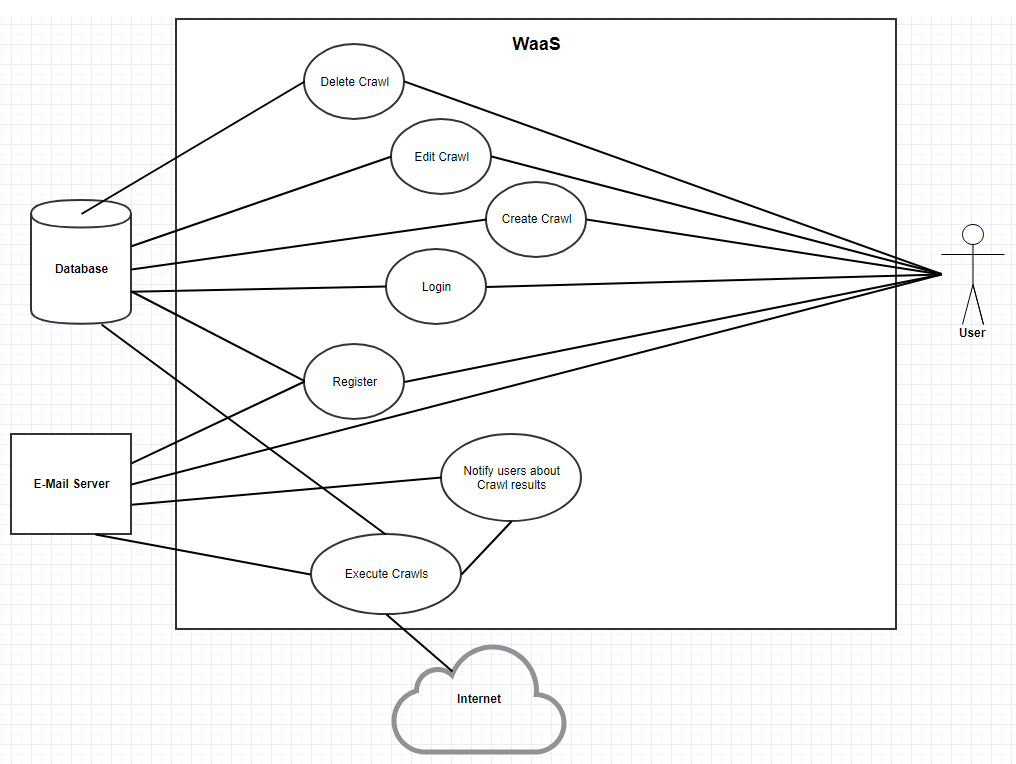
\includegraphics[width=0.95\linewidth]{UseCaseDiagram.PNG}
  \caption{Use Case Diagram}
  \label{fig:useCaseDiagram}
\end{figure}

\subsection{Functional Requirements}

The following chapter contains the functional requirements for WaaS.

\subsubsection{Target Group}

The target group of WaaS are mainly people that are regularly checking websites for news. That concludes people of all ages who understand what a web scraper is. It can also be used from people who want to check wether or not the new episode of their favourite tv series is already online. All of those people are generally expected to have some basic skills in the field of IT or are at least interested in it.

\subsubsection{{Use Cases}}

\begin{table}[H]
  \begin{center}

    \begin{tabular}{p{4cm}|p{10cm}}
      \textbf{UST-1}   & \textbf{Register}                                                                                            \\
      \hline
      Goal             & A user registers a user account for WaaS.                                                                    \\
      \hline
      Actors           & Eventual user of WaaS                                                                                        \\
      \hline
      Precondition     & The user owns a valid email address that is not yet used for an existing user account                        \\
      \hline
      Trigger          & Click on the button: "Register"                                                                              \\
      \hline
      Main path        &
      \begin{packed_itemize}
        \item [1] The user clicks the button: "SignUp".
        \item [2] The user enters his credentials into the register form (email address, and password).
        \item [3] The user clicks on: "Register".
        \item [4] WaaS creates a user account entry in the database.
        \item [5] The user gets redirected to the Login Page.
      \end{packed_itemize}                                                                                                       \\
      \hline
      Alternative path &
      \begin{packed_itemize}
        \item [1a] The user enters a invalid input data.
        \item [2a] A validation error message shows up.
      \end{packed_itemize}                                                                                                       \\
      \hline
      Postcondition    & A new user account was created in the database with the credentials the user entered into the register form. \\
    \end{tabular}

    \caption{UST-1}
    \label{table:UST-1}

  \end{center}
\end{table}

\begin{table}[H]
  \begin{center}

    \begin{tabular}{p{4cm}|p{10cm}}
      \textbf{UST-2}   & \textbf{Login}                                                 \\
      \hline
      Goal             & A user logs in with an existing user account.                  \\
      \hline
      Actors           & registered users                                               \\
      \hline
      Precondition     & UST-\ref{table:UST-1}                                          \\
      \hline
      Trigger          & Click on the button: "LogIn"                                   \\
      \hline
      Main path        &
      \begin{packed_itemize}
        \item [1] The user enters a valid email address an password into the login form.
        \item [2] The user clicks on the button: "LogIn".
      \end{packed_itemize}                                                         \\
      \hline
      Alternative path &
      \begin{packed_itemize}
        \item [1a] The user enters a invalid input data.
        \item [2a] A validation error message shows up.
      \end{packed_itemize}                                                         \\
      \hline
      Postcondition    & The user is now logged in and is situated on the overview page \\
    \end{tabular}

    \caption{UST-2}
    \label{table:UST-2}

  \end{center}
\end{table}

\begin{table}[H]
  \begin{center}

    \begin{tabular}{p{4cm}|p{10cm}}
      \textbf{UST-3}   & \textbf{Create Scrape}                                                                                             \\
      \hline
      Goal             & A user creates a new scrape.                                                                                       \\
      \hline
      Actors           & logged in users                                                                                                    \\
      \hline
      Precondition     & UST-\ref{table:UST-1} \& UST-\ref{table:UST-2}                                                                     \\
      \hline
      Trigger          & Click on the button: "+"                                                                                           \\
      \hline
      Main path        &
      \begin{packed_itemize}
        \item [1] The user enters a URL into the New Scrape form.
        \item [2] The form shows if the entered URL is valid.
        \item [3] The user enters a Scrape pattern into the New Scrape form.
        \item [4] The user clicks on the button: "Save".
      \end{packed_itemize}                                                                                                             \\
      \hline
      Alternative path &
      \begin{packed_itemize}
        \item [1a] The user clicks the button "Cancel".
      \end{packed_itemize}                                                                                                             \\
      \hline
      Postcondition    & The newly created scrape is persisted in the database \& The new scrape gets displayed on the users overview page. \\
    \end{tabular}

    \caption{UST-3}
    \label{table:UST-3}

  \end{center}
\end{table}

\begin{table}[H]
  \begin{center}

    \begin{tabular}{p{4cm}|p{10cm}}
      \textbf{UST-4}   & \textbf{Delete Scrape}                                                                                           \\
      \hline
      Goal             & A user deletes an existing scrape.                                                                               \\
      \hline
      Actors           & logged in user                                                                                                   \\
      \hline
      Precondition     & UST-\ref{table:UST-3}                                                                                            \\
      \hline
      Trigger          & Click on the delete scrape button.                                                                               \\
      \hline
      Main path        &

      \begin{packed_itemize}
        \item [1] The user clicks on the delete button of the scrape he wishes to remove.
        \item [2] A confirmation dialogue is shown.
        \item [3] The user clicks the "Delete" button.
        \item [4] The scrape gets deleted from the database.
      \end{packed_itemize}                                                                                                          \\
      \hline
      Alternative path &
      \begin{packed_itemize}
        \item [3a] The user clicks the button "Cancel".
        \item [4a] The confirmation dialogue closes.
      \end{packed_itemize}                                                                                                          \\
      \hline
      Postcondition    & The scrape is deleted from the database \& The scrape does not get displayed on the users overview page anymore. \\
    \end{tabular}
    \vspace{-2mm}
    \caption{UST-4}
    \label{table:UST-4}

  \end{center}
\end{table}

\begin{table}[H]
  \begin{center}

    \begin{tabular}{p{4cm}|p{10cm}}
      \textbf{UST-5}   & \textbf{Edit Scrape}                                    \\
      \hline
      Goal             & A user edits an existing scrape.                        \\
      \hline
      Actors           & logged in user                                          \\
      \hline
      Precondition     & UST-\ref{table:UST-3}                                   \\
      \hline
      Trigger          & Click on the edit scrape button.                        \\
      \hline
      Main path        &
      \begin{packed_itemize}
        \item [1] The user clicks on the edit button of the Scrape he wishes to edit.
        \item [2] The Edit Scrape form is shown.
        \item [3] The user changes the Scrape's URL.
        \item [4] The form shows if the entered URL is valid.
        \item [5] The user clicks "Save".
        \item [6] The changes get persisted in the database.
      \end{packed_itemize}                                                 \\
      \hline
      Alternative path &
      \begin{packed_itemize}
        \item [2a] The user clicks the button "Cancel".
        \item [3a] The Edit Scrape form closes.
      \end{packed_itemize}                                                 \\
      \hline
      Postcondition    & The updated Scrape gets displayed on the overview page. \\
    \end{tabular}

    \vspace{-2mm}
    \caption{UST-5}
    \label{table:UST-5}

  \end{center}
\end{table}

\begin{table}[H]
  \begin{center}

    \begin{tabular}{p{4cm}|p{10cm}}
      \textbf{UST-6}                & \textbf{Receive and Dismiss Notification}                    \\
      \hline
      Goal                          & A user gets notified about a Scrape having been triggered.   \\
      \hline
      Actors                        & user                                                         \\
      \hline
      Precondition                  & UST-\ref{table:UST-3}                                        \\
      \hline
      Trigger                       & WaaS found defined Scrape pattern on Scrape URL.             \\
      \hline
      Main path                     &
      \begin{packed_itemize}
        \item [1] The user receives an E-Mail notifying him about the triggered Scrape.
        \item [2] The user clicks on the link in the E-Mail.
        \item [3] The notification gets dismissed by the system.
        \item [4] The user gets redirected to the URL of the Scrape.
      \end{packed_itemize}                                                                   \\
      \hline
      Alternate path:                                                                              \\
      Notification Tray             &
      \begin{packed_itemize}
        \item [1a] The user logs in to WaaS.
        \item [1b] The user opens the notification tray.
        \item [2a] The user clicks on the notification in the tray
      \end{packed_itemize}                                                                   \\
      \hline
      Alternate path:                                                                              \\
      Notification Tray Dismiss All &
      \begin{packed_itemize}
        \item [1a] The user logs in to WaaS.
        \item [1b] The user opens the notification tray.
        \item [2a] The user dismisses all notifications.
        \item [3a] All previously unread notifications get marked read.
      \end{packed_itemize}                                                                   \\
      \hline
      Postcondition                 & The user has been notified about his scrape being triggered. \\
    \end{tabular}

    \vspace{-2mm}
    \caption{UST-6}
    \label{table:UST-6}

  \end{center}
\end{table}

\begin{table}[H]
  \begin{center}

    \begin{tabular}{p{4cm}|p{10cm}}
      \textbf{UST-7} & \textbf{Show Scrape History}                      \\
      \hline
      Goal           & A user can see all past triggers of a Scrape.     \\
      \hline
      Actors         & logged in user                                    \\
      \hline
      Precondition   & UST-\ref{table:UST-3}                             \\
      \hline
      Trigger        & User opens Scrape details.                        \\
      \hline
      Main path      &
      \begin{packed_itemize}
        \item [1] The opens the Scrape details.
        \item [2] Details include an overview of past triggers for the Scrape.
      \end{packed_itemize}                                         \\
      \hline
      Postcondition  & The user has gotten information about his Scrape. \\
    \end{tabular}

    \vspace{-2mm}
    \caption{UST-7}
    \label{table:UST-7}

  \end{center}
\end{table}

\subsection{Non-functional Requirements}

\begin{enumerate}
  \item \textbf{Performance}
        \begin{enumerate}
          \item For user interactions, the application should respond 99\% of the requests in 2 seconds.
          \item The application should score at least 40 points of performance in Google Chromes inbuilt Lighthouse audit.
        \end{enumerate}
  \item \textbf{Usability}
        \begin{enumerate}
          \item If the application experiences any kind of error or delay, users should be made aware of this.
          \item When a website that is subject to a Scrape changes to contain the looked for pattern, users should receive a notification within an hour.
        \end{enumerate}
  \item \textbf{Other non-functional requirements}
        \begin{enumerate}
          \item The application should be implemented according to best practices and should therefore score 100 points in the best practices section of the Lighthouse audit.
          \item Due to the use of relational database technology, horizontal scalability is too big of a task to be realized in the given time frame and is therefore outside of the scope of this project.
        \end{enumerate}
\end{enumerate}

\section{GUI and Navigation Design}
\subsection{Navigation Model}

The following diagram depicts principal states and possible user interactions to navigate between them.

\begin{figure}[H]
  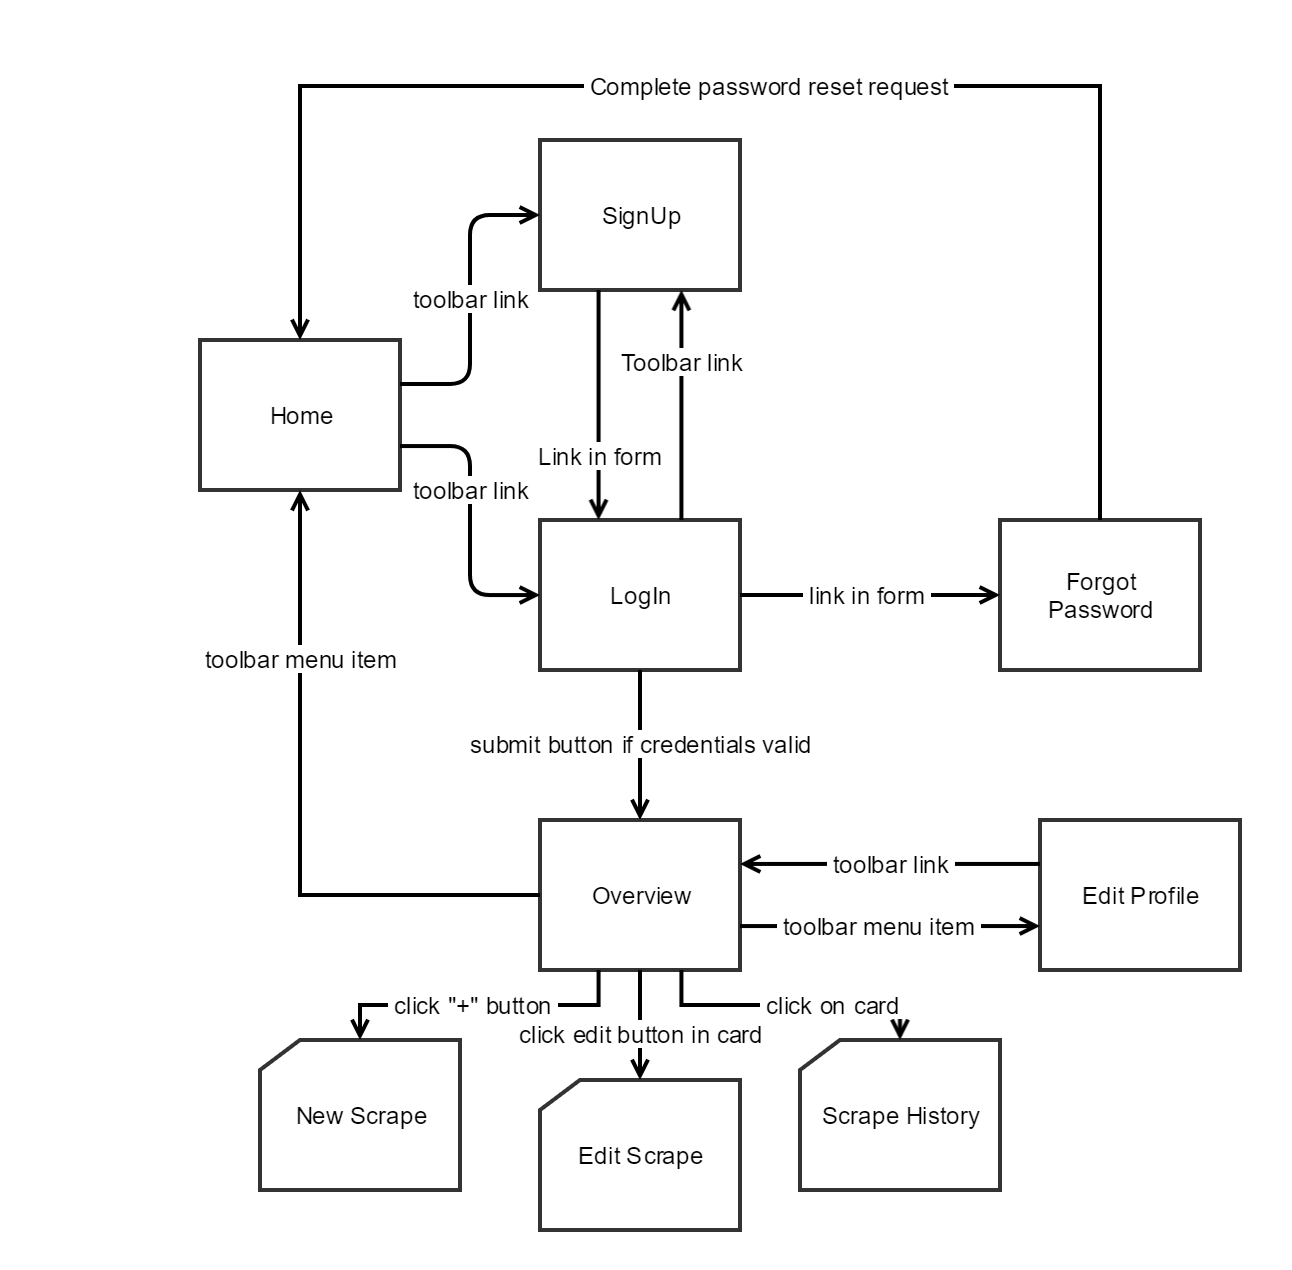
\includegraphics[width=0.95\linewidth]{navigationmodel_waas.png}
  \caption{Navigation Model}
  \label{fig:navigationModel}
\end{figure}

The boxes represent states and the arrows the means to transition from one state to another. The boxes with a missing corner represent a modal and the arrows leading up to the modals aren't state transitions since the modals don't
represent a complete state but a GUI element within their parent state. The modal blocks other interactions until it is dismissed, either through cancelling it or following through on its action. \\
The user enters the page on "Home" and needs to log in to get to the main state called "Overview". From there, all other interactions to manage Scrapes are possible.

\subsubsection{Potential sources of errors}
The following issues may arise from the navigation.

\paragraph{User doesn't want to register}
It is possible, that a user wants to see how WaaS works, without registering beforehand.
This is not possible in the navigation model since a user needs to be logged in to use WaaS. Since it is possible for users to delete their accounts it is a minor issue though.

\paragraph{User gets lost in a branch state}
A user could get lost in a state because he doesn't see, how to leave it. Usually, a user will then use the browsers back button, so it's important to either make sure it works or to offer the user an obvious alternative back action.

\paragraph{User may not know that a click on a card shows the scrape history}
It may not be intuitive for some users to click on a card in order to display the history of a scrape. If this turns out to be a problem it could be solved by adding a button for the history.

\subsubsection{Automation in Navigation Design}

Once a navigation design was created, it can be useful to analyze it in order to find potential errors and bad design choices. For a small application where the navigation design is not that complex this can easily be achieved by hand. For more complex navigation models this may be difficult to do \cite{mSharonHurleyHall2019}. Therefore a variety of tools can be used to automate this process. One possible choice is Google Analytics. If there already is an existing website or an html prototype google analytics can visualize user flows and direct you to potential problems in the navigational design as described in this article \cite{mAndyCrestodina2018}.

Since WaaS is a rather small and simple application we found it unnecessary to do automated analytics of our navigation design.

\subsection{HTML Prototype}
To visualize the navigation model, a HTML Prototype was created and is available either in the adjacent documents to this documentation or through the GitHub Page on \url{https://nipfi.github.io/ffhs-WebE/HTML%20Prototype/index.html}.

\pagebreak

\listoftablesö
\listoffigures

\pagebreak

\bibliography{uni}
\bibliographystyle{ieeetr}


\end{document}
